\documentclass[12pt]{article}
\usepackage{amsfonts,amsthm,amsmath,amssymb,mathtools}
\usepackage{mathrsfs}
\usepackage{enumitem}
\usepackage{tikz-cd}
\usepackage{geometry}
\usepackage{mlmodern}
\usepackage{graphicx}

\geometry{letterpaper, portrait, margin=1in}

\setcounter{section}{0}

\renewcommand{\thesection}{\S\arabic{section}}
\renewcommand{\thesubsection}{\arabic{section}}
\DeclareMathOperator{\im}{im}

\newtheorem{thm}{Theorem}
\newenvironment{theorem}[1]{
	\renewcommand{\thethm}{#1}
	\begin{thm}
		}{\end{thm}}

\newtheorem{lma}{Lemma}
\newenvironment{lemma}[1]{
	\renewcommand{\thelma}{#1}
	\begin{lma}
		}{\end{lma}}

\theoremstyle{definition}
\newtheorem{ex}{Assignment}
\newenvironment{exercise}[1]{
	\renewcommand{\theex}{#1}
	\begin{ex}
		}{\end{ex}}

\title{MTH 732 Topology - Homework 4}
\author{Connor Mooneyhan}
\date{February 12, 2026}

\begin{document}

\maketitle

\begin{ex}
	Compute the fundamental group of $\mathbb{R}^2$ with two points removed.
\end{ex}
\begin{proof}
	(Note: all disk boundaries pictured in this proof are understood to be open.)\\
	We can view this homeomorphically as $\mathrm{int}(D^2)$ with two points removed:\\
	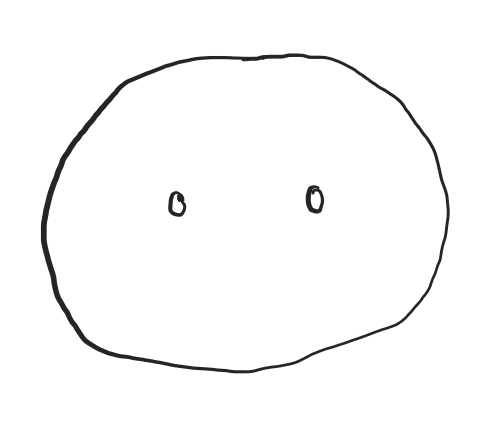
\includegraphics[width=0.4\textwidth]{one-disk}\\
	We can break this up into two open disks $U$ and $V$, each with one point removed:\\
	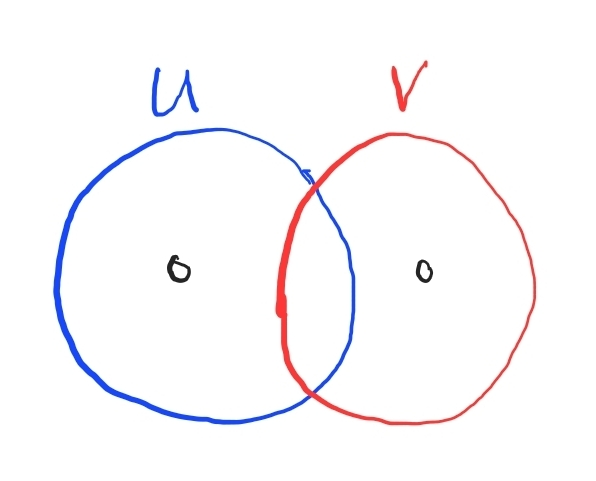
\includegraphics[width=0.4\textwidth]{two-disks}\\
	We know that $\pi_1(U) = \left\langle a \right\rangle$ and $\pi_1(V) = \left\langle b \right\rangle$ while $\pi_1(U \cap V)$ is trivial.
	Then we can use Seifert-van Kampen to get \begin{equation*}
		\pi_1(U \cup V) = \left\langle a, b \right\rangle.
	\end{equation*}
\end{proof}

\begin{ex}
	If $F \subset \mathbb{R}^3$ is a finite set, show that $\mathbb{R}^3 \setminus F$ is simply-connected.
\end{ex}
\begin{proof}
	Let $n$ be the size of $F$, and define $F_n = \left\lbrace (0, 0, 0), \dots, (n - 1, 0, 0) \right\rbrace$.
  Also, define $B^3 = \mathrm{int}(D^3)$ centered at the origin.
	We can then model $\mathbb{R}^3 \setminus F$ homeomorphically as $\mathbb{R}^3 \setminus F_n$.
  Clearly $\mathbb{R}^3 \setminus F_n$ is path-connected, so we will focus on the fundamental groups.

  First, when $n = 1$, $\mathbb{R} \setminus F_n$ has $S^2$ as a deformation retract, which we know to have trivial fundamental group.
  The same is true for $B^3 \setminus F_n$ in this case since it is also a deformation retract of $\mathbb{R}^3$.
  Now assume we have proven the hypothesis through $n - 1$, and define $C = \left\lbrace (x, y, z) : x^2 + y^2 + z^2 > 0.9 \right\rbrace$.
  Then we can express $\mathbb{R}^3 \setminus F_n$ as a union of $B^3 \setminus F_1$ with $C \setminus F_{n-1}$.
  Luckily, $C \setminus F_{n-1}$ is homotopy equivalent to $B^3 \setminus F_{n-1}$, and since $(B^3 \setminus F_1) \cap (C \setminus F_{n-1})$ is homotopy equivalent to $S^2$, we know everything we need for Seifert-van Kampen.
  Since all the fundamental groups in question are trivial, so is $\pi_1(\mathbb{R}^3 \setminus F)$.
\end{proof}

\begin{ex}
	Compute the fundamental group of the following graph:\\
	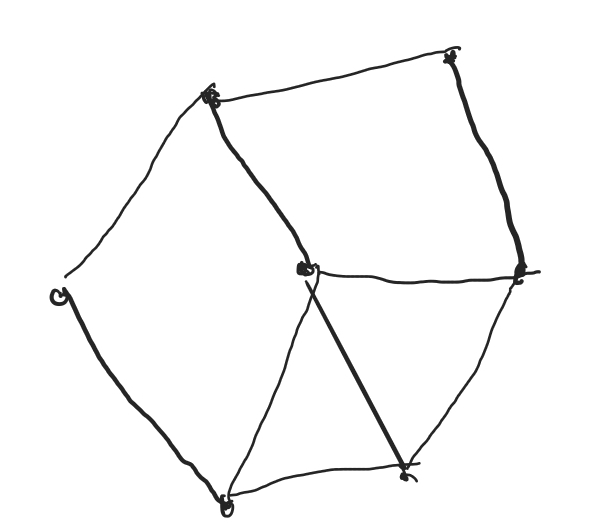
\includegraphics[width=0.4\textwidth]{initial-graph}
\end{ex}
\begin{proof}
	Consider the deformation retract pictured, where the red spanning tree is contracted to a point:\\
	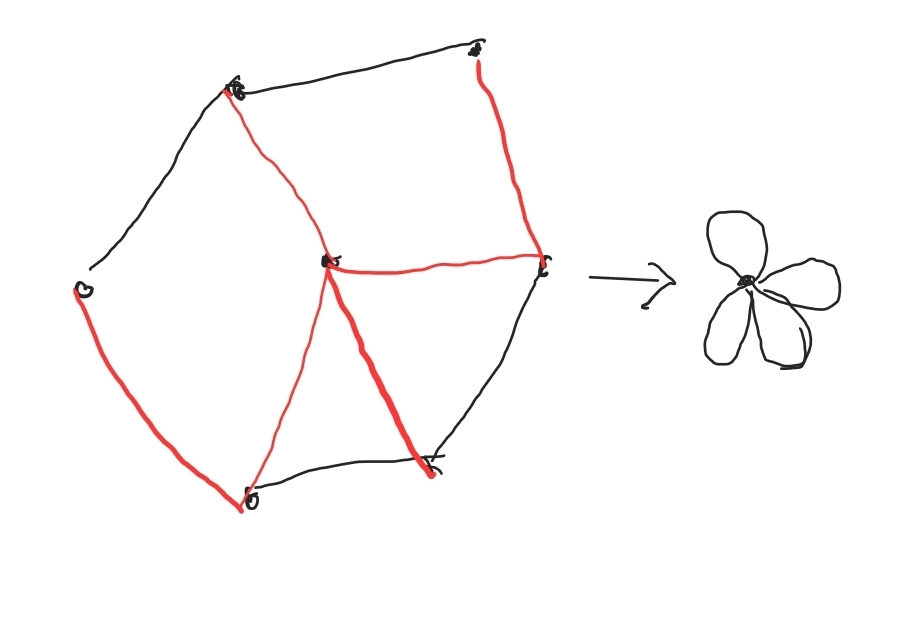
\includegraphics[width=0.4\textwidth]{contraction}\\
	Thus the graph has the same fundamental group as a wedge of four circles, which is the free group on four generators.
\end{proof}

\begin{ex}
	Let $X$ be the union of $n$ lines through the origin in $\mathbb{R}^3$.
	Compute the fundamental group of its complement $\pi_1(\mathbb{R}^3 - X)$.
\end{ex}
\begin{proof}
	Note that since, in particular, the origin is not in $\mathbb{R}^3 - X$, we can deformation retract this space to the unit sphere with $2n$ points removed.
	We can compute the fundamental group, then, by expressing it as the union of two punctured open discs $U$ and $V$, say where $z > -0.1$ and $z < 0.1$ respectively.
	Furthermore, we can consider $U \setminus V$ to contain exactly one of the points and $V \setminus U$ to contain all $2n - 1$ others (which can be achieved by homeomorphism).

	First, note that $U \cap V$ is the ``open band'' or annulus $S^2 \cap \left\lbrace (x, y, z) : -0.1 < z < 0.1 \right\rbrace$, so $\pi_1(U \cap V)$ is the free group on one generator $\gamma$.
	Also, $\pi_1(U)$ is the free group on one generator, say $\alpha$, and $\pi_1(V) = \left\langle \beta_1, \dots, \beta_{2n-1} \right\rangle$.
	Finally, the image of $\gamma$ induced by inclusion into $U$ and $V$ is $\alpha$ and $\beta_1 * \cdots * \beta_{2n-1}$ respectively, since it represents a loop running along/near the outer edges of $U$ and $V$.
	Seifert-van Kampen tells us, then (since all of these are path-connected), that \begin{align*}
		\pi_1(\mathbb{R}^3 - X) & = \pi_1(U \cup V)                                                                                            \\
		                        & = \left\langle \alpha, \beta_1, \dots, \beta_{2n-1} : \alpha = \beta_1 * \cdots * \beta_{2n-1} \right\rangle \\
		                        & = \left\langle \beta_1, \dots, \beta_{2n-1} \right\rangle.
	\end{align*}
	Thus $\pi_1(\mathbb{R}^3 - X)$ is the free group on $2n-1$ generators.
\end{proof}

\begin{ex}
	Compute the fundamental group of the connected sum \begin{equation*}
		\mathbb{RP}^2 \# \cdots \# \mathbb{RP}^2
	\end{equation*}
	of $k$ copies of the projective plane $\mathbb{RP}^2$.
\end{ex}
\begin{proof}
	As we have done before, we can use Seifert-van Kampen recursively.
	First, when $k = 2$, we can take neighborhoods $U$ and $V$ of the two copies of $\mathbb{RP}^2$ which intersect only on a small neighborhood of the disk along which they are connected.
	That intersection will have free fundamental group on one generator.
	Taking the model of $\mathbb{RP}^2$ as identifying antipodal points in $S^2$, we need to consider taking an open disk out, which is what happens when we take the connect sum.
	If we take a disk out, we can think of each copy of $\mathbb{RP}^2$ as, say, $U = S^2 \cap \left\lbrace (x, y, z) : z > -0.1 \right\rbrace$ and $V = S^2 \cap \left\lbrace (x, y, z) : z < 0.1 \right\rbrace$ under the appropriate identifications.
	Thus we can consider the generator of $\pi_1(U \cap V)$ as the equator ($z = 0$), which we know can be expressed as $a^2$ in $\pi_1(U)$ and $b^2$ in $\pi_1(V)$, where $a$ and $b$ are the usual projections of the ``halfway around the equator'' path.
	Thus \begin{equation*}
		\pi_1(\mathbb{RP}^2 \# \mathbb{RP}^2) = \left\langle a, b : a^2 = b^2 = 1 \right\rangle.
	\end{equation*}

	Repeating this calculation for a general $k$ through induction, we get \begin{equation*}
		\pi_1(\mathbb{RP}^2 \# \cdots \# \mathbb{RP}^2) = \left\langle x_1, \dots, x_k : x_1^2 = \cdots = x_k^2 = 1 \right\rangle.
	\end{equation*}
\end{proof}

\end{document}
